\section{Toy model for the prompt $\phi$ approach}
Since the decay intensity of two prompt $K_S$ is simply 
\begin{equation}
I(t_1,t_2) \propto e^{-\Gamma_S t_1}e^{-\Gamma_S t_2}, 
\end{equation} 
a toy study based on the assumption that all background consists of prompt $K_S$ has been done using RooFit. To make the model more realistic, it includes an approximate transverse momentum distribution which is shown in figure \ref{FIG:Mommodel}. 

\begin{center}
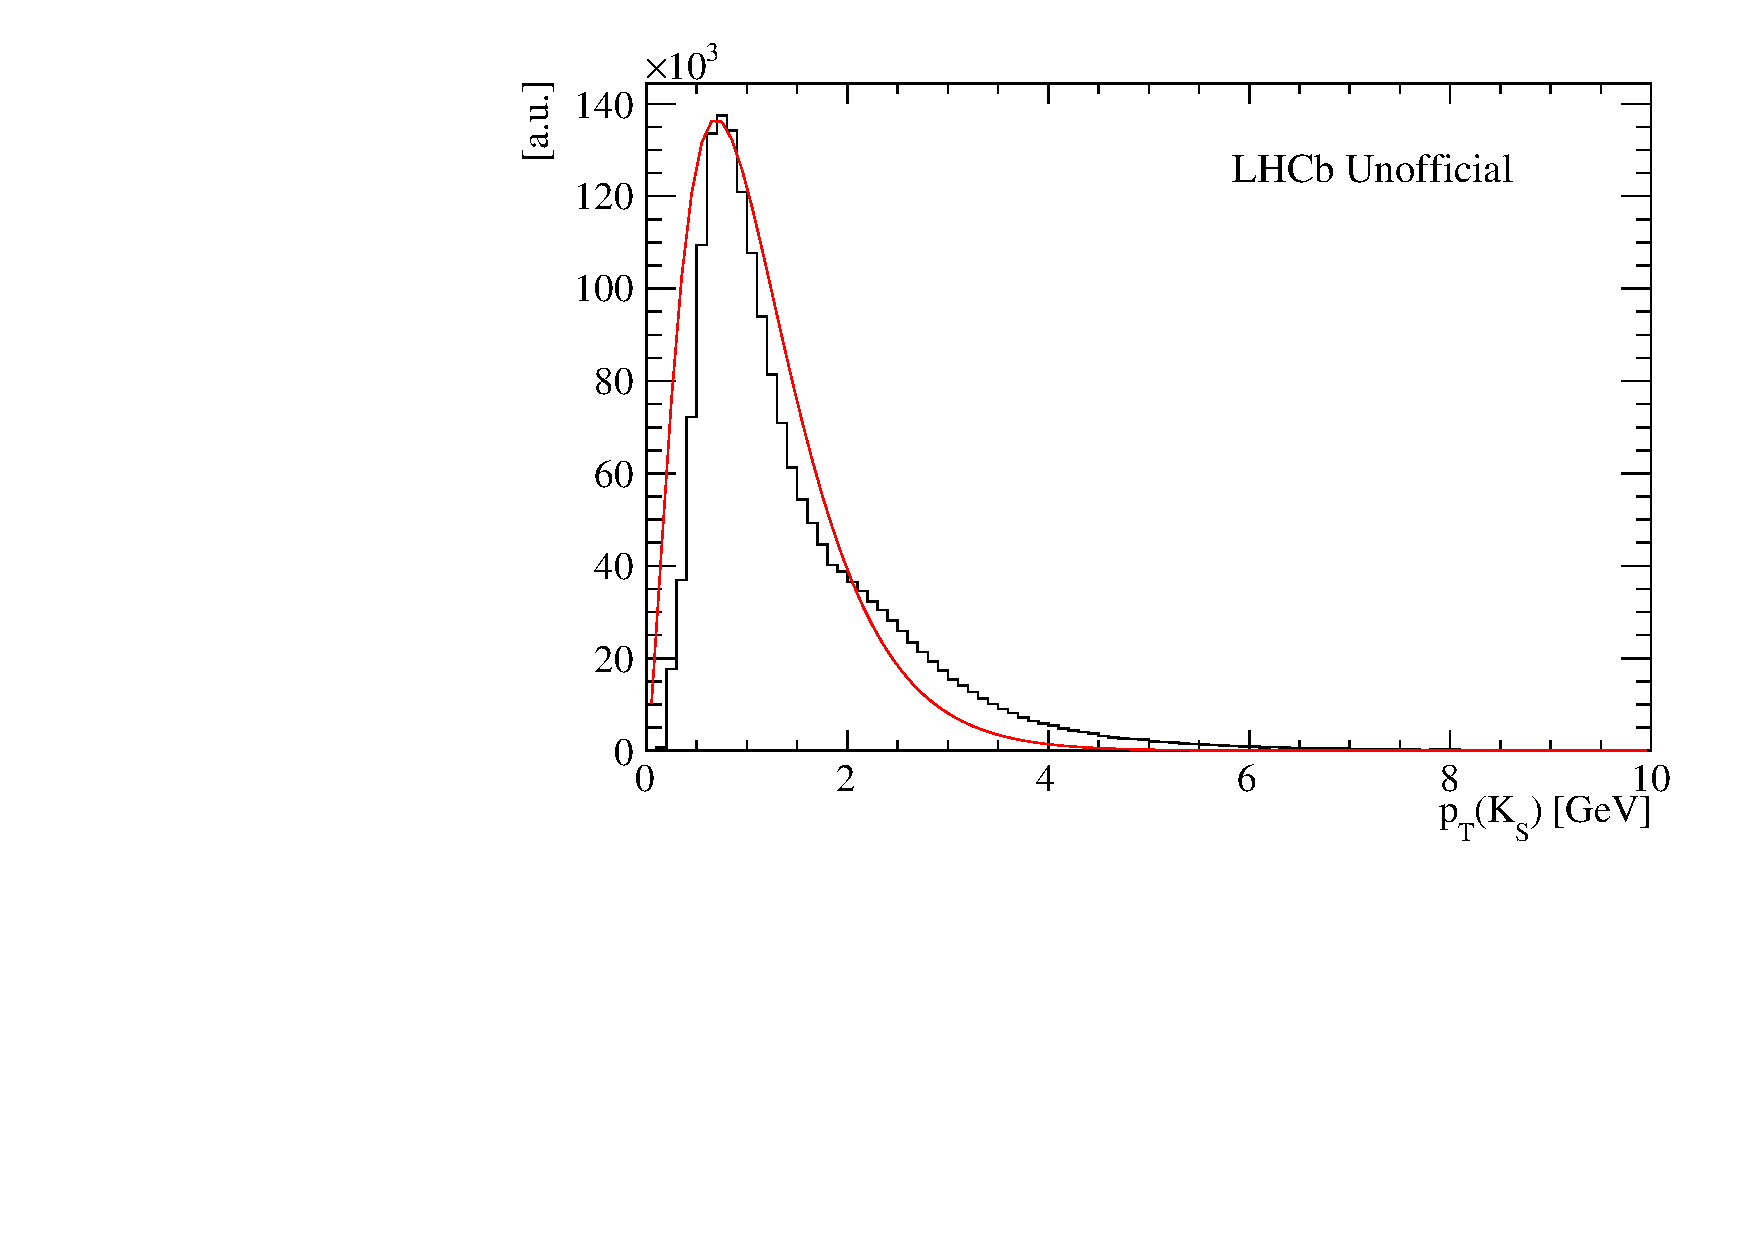
\includegraphics[height=.48\textwidth]{/home/soonja/lxplus/phi2KsKs/phi2KsKs/preliminaryStudies/mommodel.pdf}
\captionof{figure}{Transverse momentum of the kaons. The black line shows the distribution in 2012 data and the red line the approximation used in the model.}\label{FIG:Mommodel}
\end{center}

The approximative form used is
\begin{equation}
N(p_T(K_S)) \propto 
(p_T[MeV])^{1.52}\exp\left(-2.19\cdot10^{-3}p_T[MeV]\right) 
\end{equation}
It being part of the model is necessary in order to transfer the acceptance of events based on the transverse coordinates of the kaon decay vertices into the time domain that was studied. If for example both kaons decay inside the beampipe, that means that the $x$ and $y$ coordinate of their decay vertices have to be less than \SI{7}{mm}.

\begin{center}
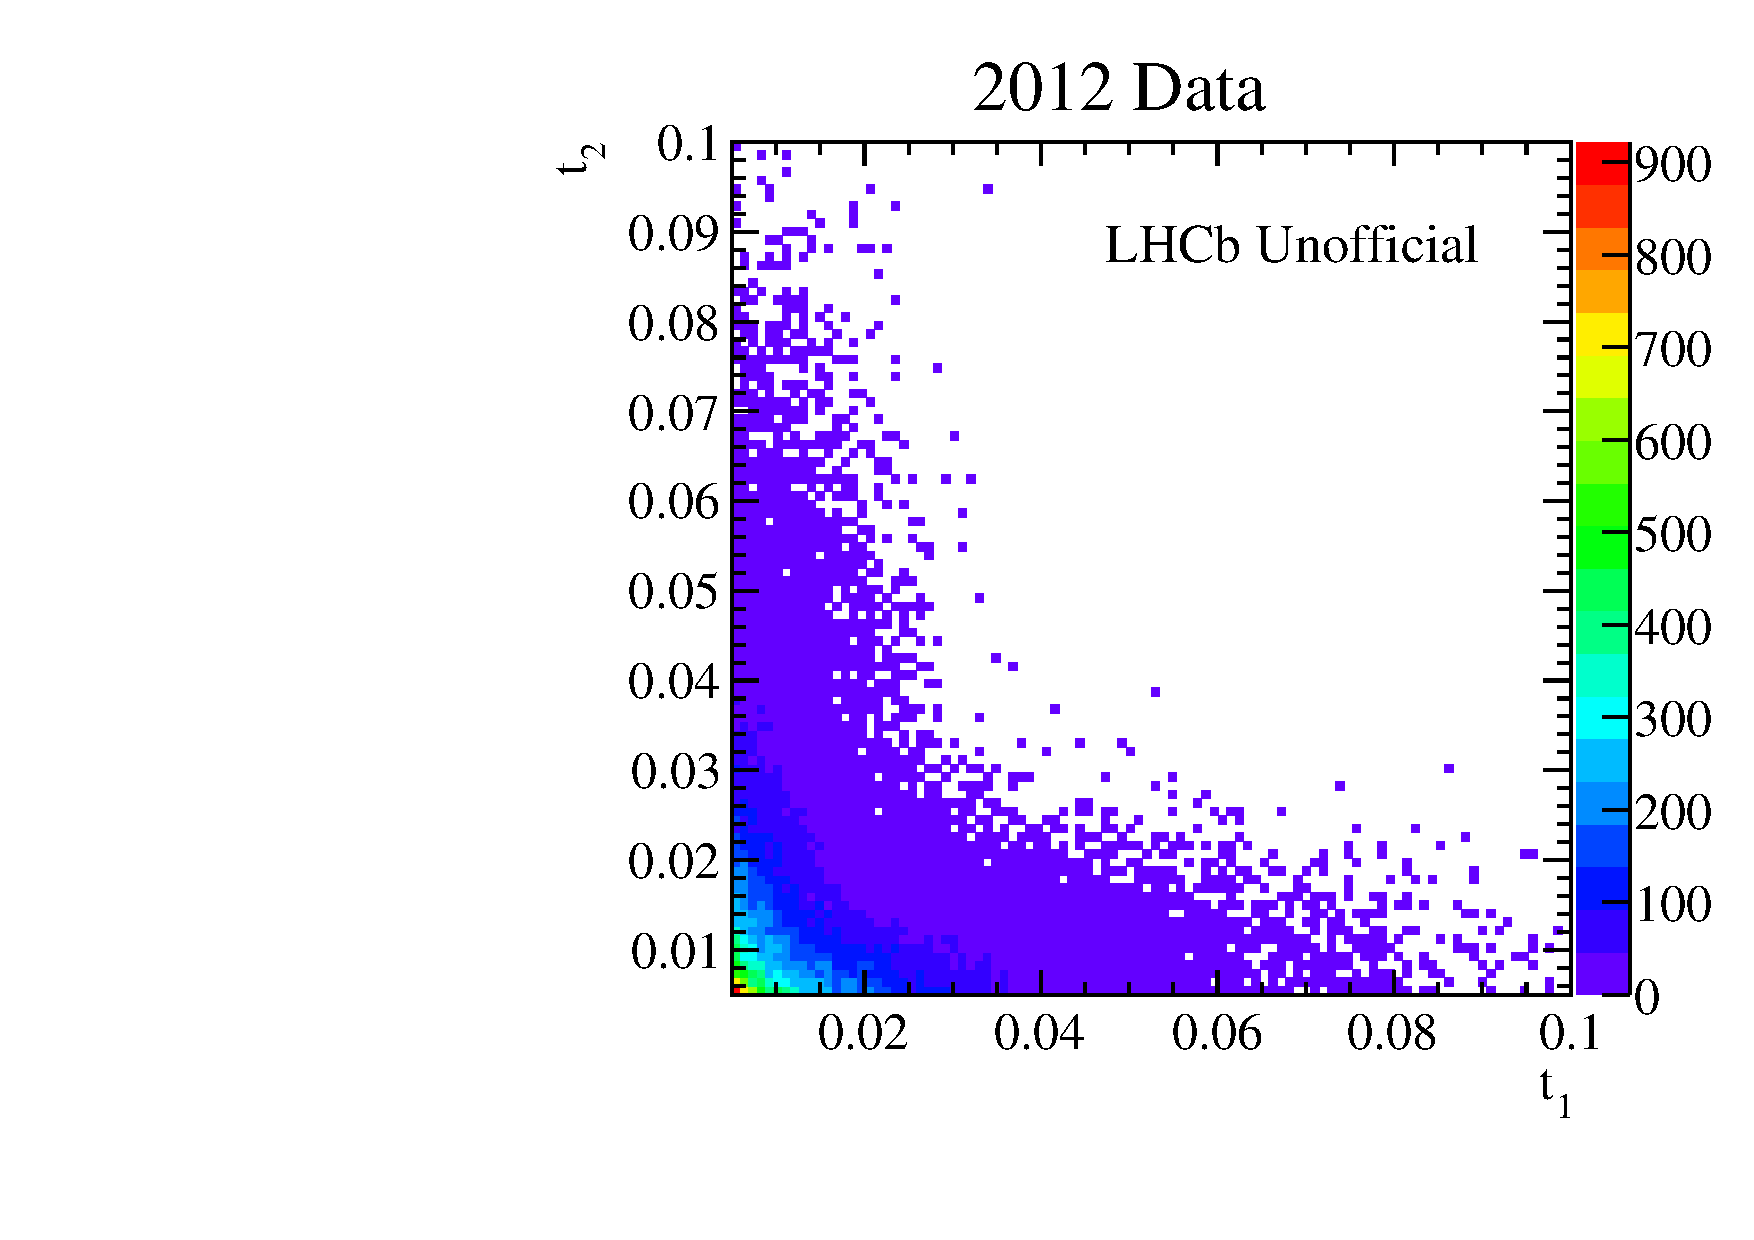
\includegraphics[width =.49\textwidth,trim= 0mm 0mm 0mm 0mm, clip]{/home/soonja/lxplus/phi2KsKs/phi2KsKs/toymodell/data.pdf}
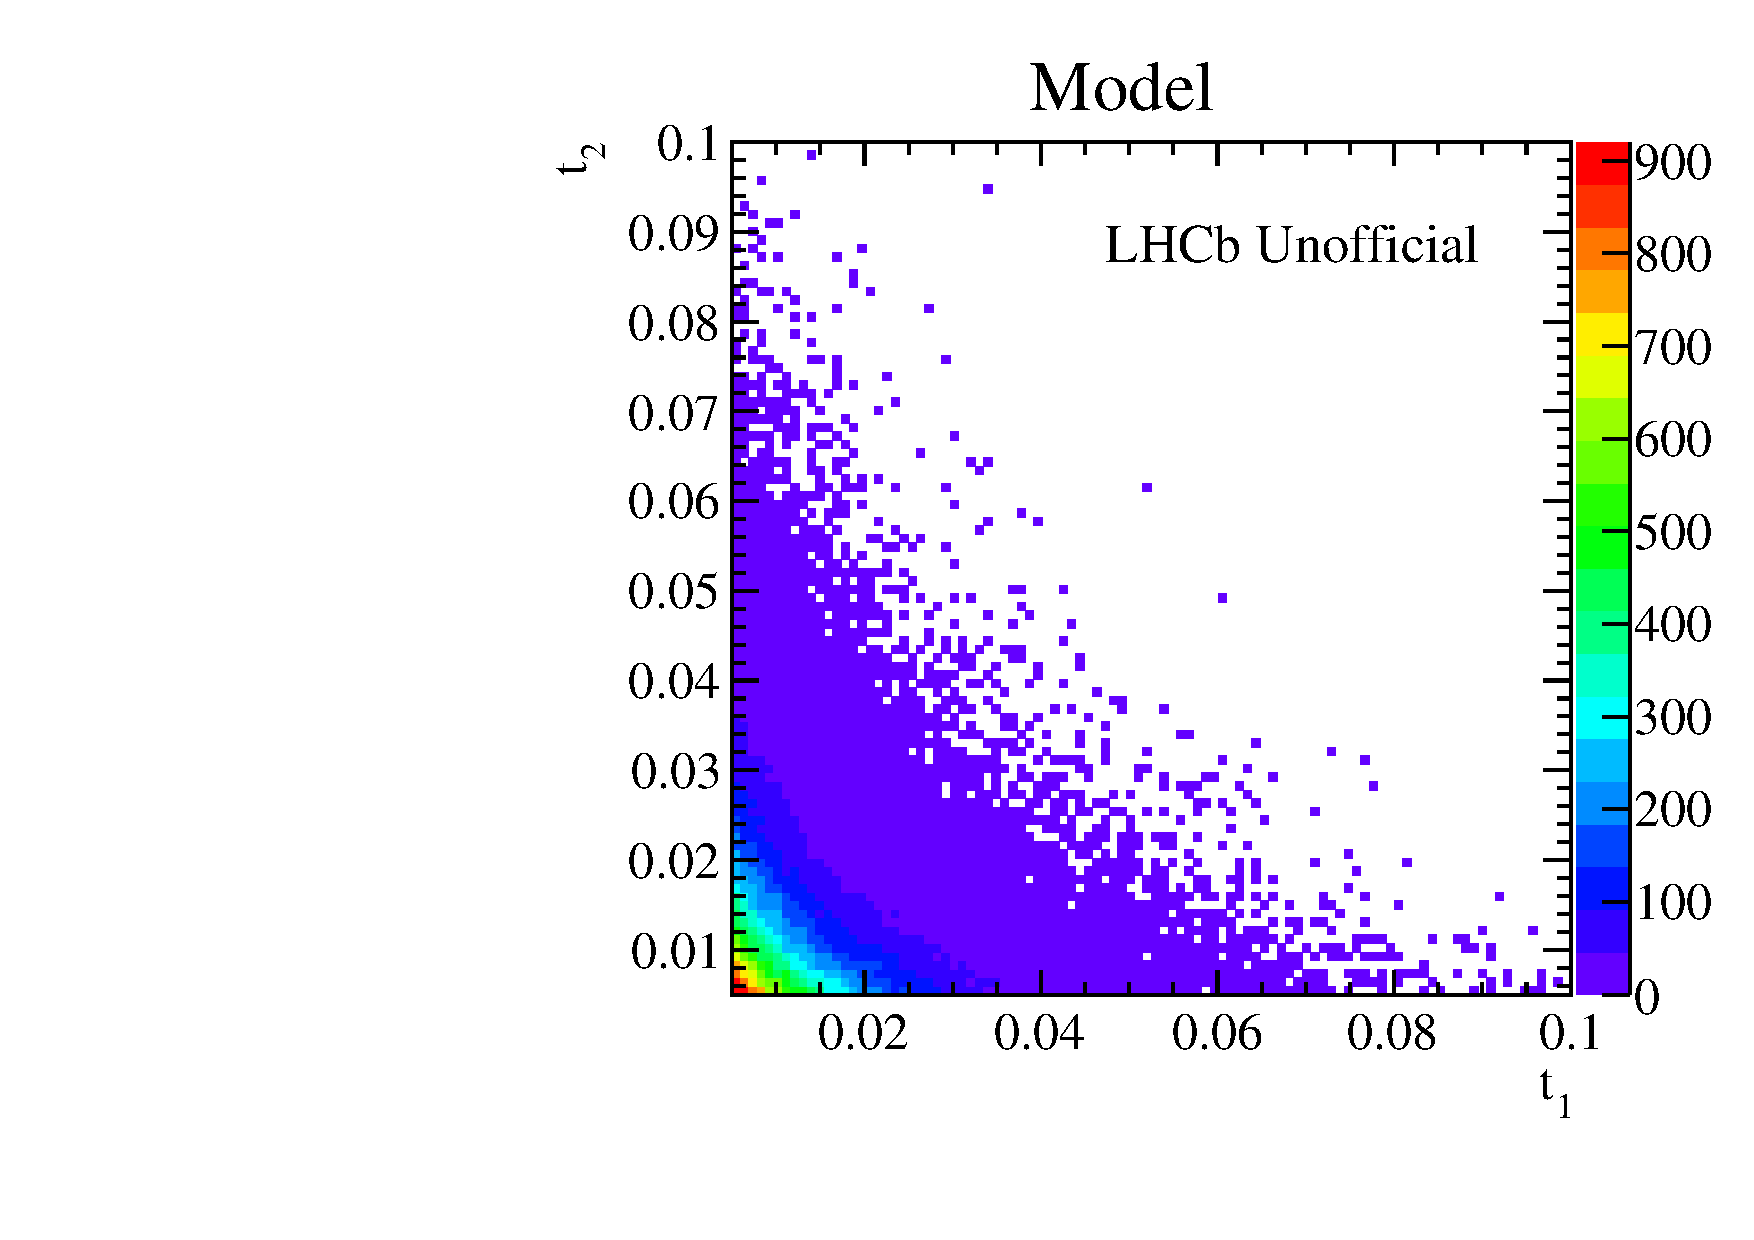
\includegraphics[width =.49\textwidth]{/home/soonja/lxplus/phi2KsKs/phi2KsKs/toymodell/model.pdf}
\captionof{figure}{Comparison between the distribution in the lifetimes of the two kaons for 2012 data and the toy model studied.}\label{FIG:2D}
\end{center}

The distribution of the decay times of the two kaons as given by the 2012 data and the model are displayed in figure \ref{FIG:2D}




A toy dataset was built by combining this model of the prompt $K_S$ with a similar one where the decay intensity of the kaons is replaced with the one given in equation \eqref{EQ:DI1} describing Standard Model background ($\zeta_{SL}=0$). They were added with weights according to a signal to background ratio of $4\cdot10^{-4}$. This ratio is an optimistic estimate gained from the efficiency study in section  \ref{SEC:Efficiencies}.



Afterwards, the RooStats profile likelihood calculator was used to determine a 95\% C.L. limit on $\zeta_{SL}$ for different luminosities based on this composite model. That was done by fitting equation \eqref{EQ:DI2} to the toy data set, leaving $\zeta_{SL}$ as a free parameter. The result is displayed in figure \ref{FIG:Limits}.

The predicted limits on $\zeta_{SL}$ go with the square root of the luminosity. The limits from the toy study have been fitted to a function with this behaviour. Based on this fit, it has been extrapolated that the necessary luminosity for being competitive with the KLOE limit $\zeta_{SL} = 0.098$ is $\int L\,dt \approx 275\,\text{fb}^{-1}$. This is far beyond the amount of luminosity planned to be collected during run II and run III.

\begin{center}
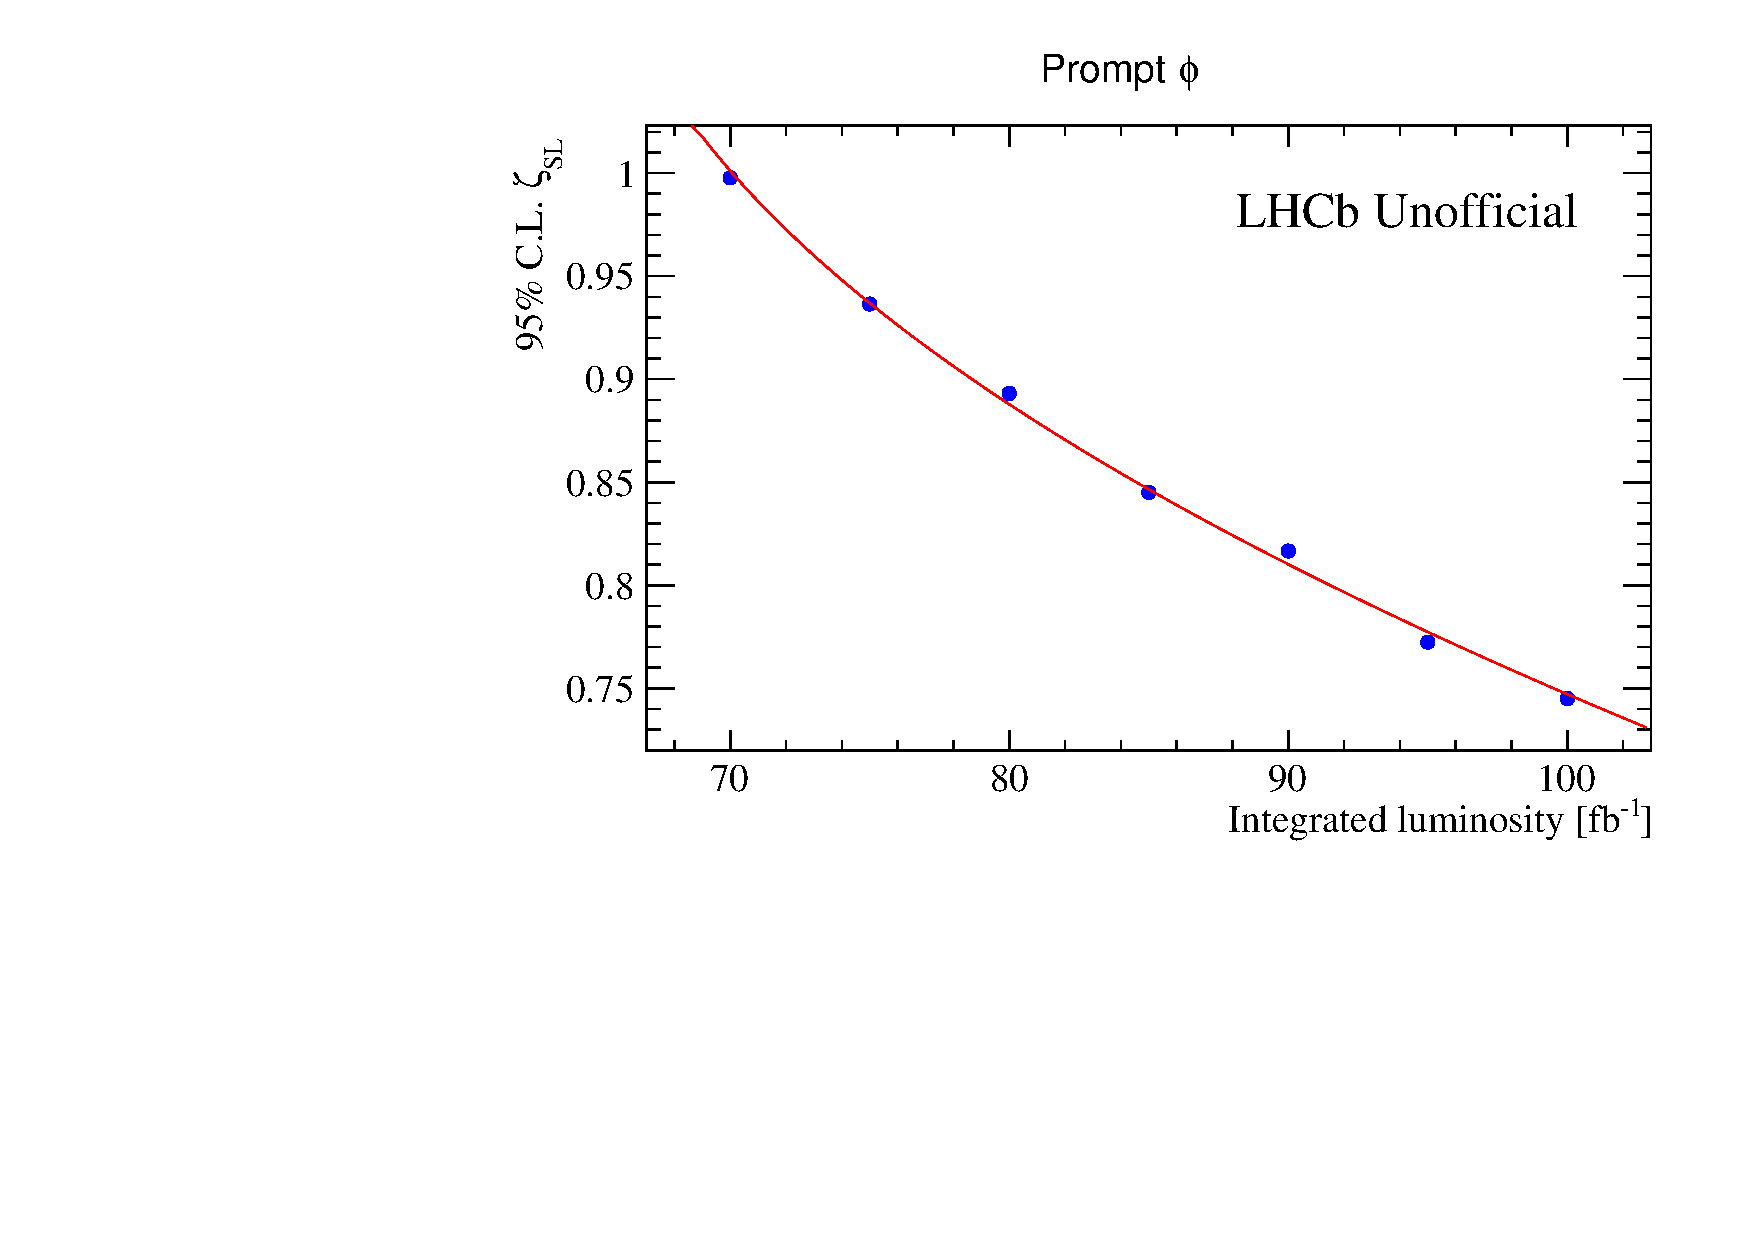
\includegraphics[width=.7\textwidth,trim= 0mm 0mm 0mm 10mm, clip]{/home/soonja/lxplus/phi2KsKs/phi2KsKs/toymodell/limits.pdf}
\captionof{figure}{Predicted 95\% C.L. limit on $\zeta_{SL}$ for the given luminosities.} \label{FIG:Limits}
\end{center}



%\item Fitted to 
%\begin{align*}
%I(t_1,t_2) \propto & e^{-\Gamma_L t_1 - \Gamma_S t_2} +e^{-\Gamma_S t_1 - \Gamma_L t_2}\\& - 2(1-\zeta_{SL}) e^{-\frac{1}{2}\left(\Gamma_S + \Gamma_L\right)\left(t_1+t_2\right)}\cos\left(\Delta m \left(t_1-t_2\right)\right)
%\end{align*}
%\item Derived limit on $\zeta_{SL}$ from fit result 
%\end{itemize}
%\end{frame}